% ==================================================%
% Basic setup starts here
%==================================================%
\documentclass[12pt, letterpaper]{amsart} % this will automatically load amsmath and amsthm packages
\usepackage{amsfonts}
\usepackage{amscd} % a CD environment for commutative rectangular diagram
\usepackage{mathtools} % for \shortintertext
\usepackage[utf8]{inputenc} % encoding method
\usepackage[mathscr]{eucal} % eucal calligraphy, mathsrc = use \mathcal
\usepackage{indentfirst} % indent first line of all sections
\usepackage{graphicx} % extension of graphics, options for \includegrahpicx
\usepackage{pict2e} % new implementation of the picture environment, which allows programming pictures directly LaTeX
\usepackage{epic} % add some command to the picture environment
\usepackage[margin=2.9cm]{geometry} % customize page layout
%==================================================%
% Additional setup ends here
%==================================================%
% Additional package used for relevant article
\usepackage{physics} % partial derivative \pdv
\usepackage{cleveref} % automatically add eq in referencing
\usepackage{cancel}
\usepackage{tikz}
\usepackage{float}
\usepackage{hyperref}
% SELF-DEFINED THEOREM using amsthm package
\newtheorem{Th}{Theorem}[section]
\numberwithin{equation}{section}
\newtheorem{Def}[Th]{Definition}
%==================================================%
% Document starts here
% ==================================================%
\author{Kin Chang \\ 304-845-848}
\title{EE183 Lab 1}
\begin{document}
\maketitle
\section{Introduction}
\begin{center}
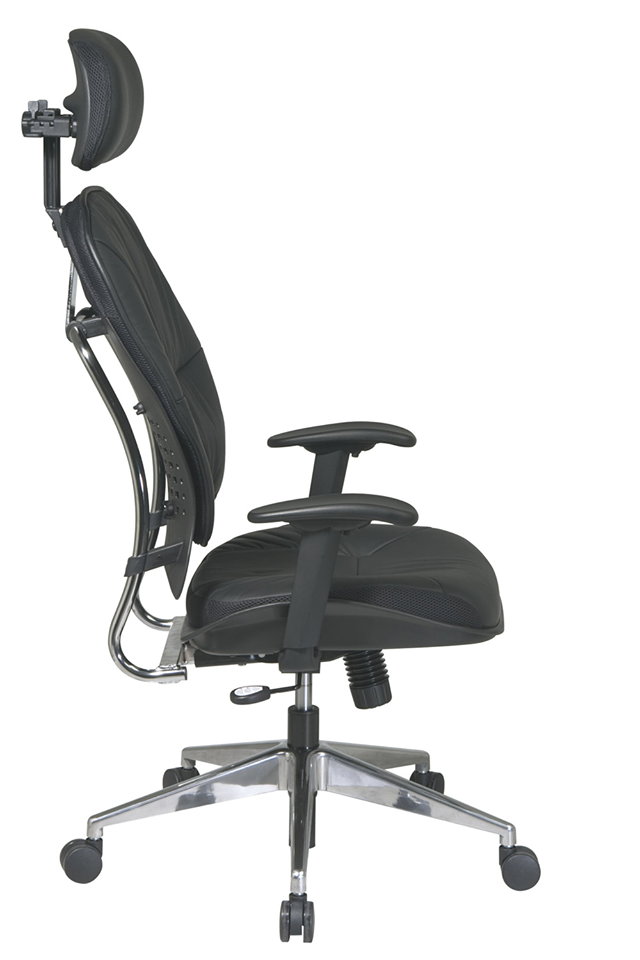
\includegraphics[scale=0.5]{1}  
\end{center}
In this lab, we model a chair with 4 joints with end effector being the headrest. A simplified model schematic of the robot is shown below,
\begin{figure}[H]
  \centering
  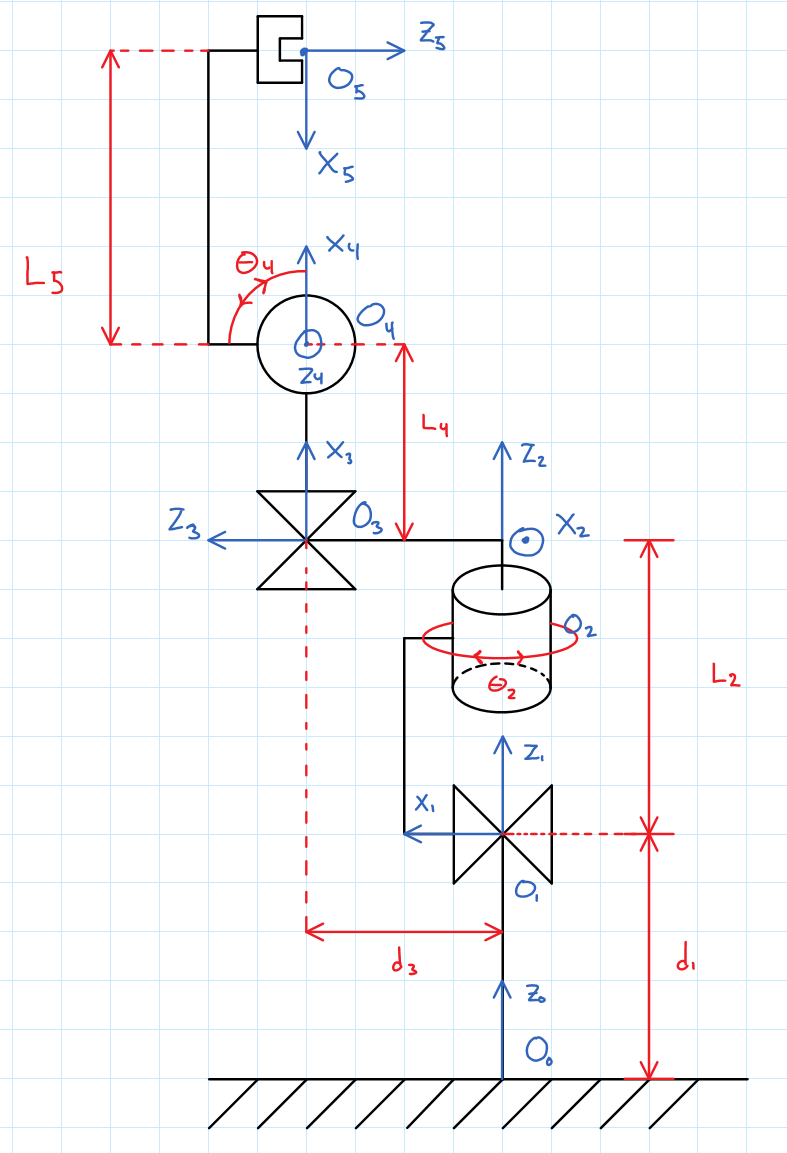
\includegraphics[scale=0.4]{image4}
  \caption{Schematic of the model}
  \label{fig:1}
\end{figure}


According the the schematic, from bottom to top, a prismatic joint is responsible for the height of the seat (along $z_1$). A revolute joint right above it rotate the chair about the $z_2$  so that person sitting on can turn their body around their environment. Another prismatic joint moves along $z_3$ axis adjusts how far back the backpanel is. Next, a revolute joint rotating about $z_4$ is responsible for adjusting the back angle the person want to sit at. Lastly, we chose the end effector to be the headrest of the chair whose positional state changes if any of the above joint variables change.
\par
This linkage has 4 degree of freedom, namely translation along z and x, and rotational about z and y in the $O_o$ world reference. The ultimate goal of this linkage is to position the headrest (in turn the back and orientation of the whole chair) in the most comfortable position for the human sitting on it.
\par
A simple case scenario in words is describe below: A human sitting on this chair facing the $-x_0$ direction wants to sit facing forward, while wants to sit higher and lean his back a little bit to the back. Intuitively, if we are to do it, this would translate to the operation on the joint:
\begin{enumerate}
\item joint 1 moves along $z_1$ by $q_1$ mm  
\item joint 2 rotates about $z_2$ by 90 degrees
\item joint 4 rotates along $z_4$ by $q_4$ degrees.  
\end{enumerate}

\section{Method}
Based off the schematic in figure 1, we computed the Denavit–Hartenberg parameters, as shown in the following table,
\begin{table}[H]
  \centering
  \begin{tabular}{c|cccc}
i & $\alpha$$_{\text{i-1}}$ & a$_{\text{i-1}}$ & d$_{\text{i}}$ & $\theta$$_{\text{i}}$\\
\hline
1 & 0 & 0 & d$_{\text{1}}$ & 0\\
2 & 0 & 0 & L$_{\text{2}}$ & $\theta_2$+90\\
3 & 90 & 0 & d$_{\text{3}}$ & 90\\
4 & 90 & L$_{\text{4}}$ & 0 & $\theta$$_{\text{4}}$\\
5 & 90 & L$_{\text{5}}$ & 0 & 180\\
\end{tabular}
  \caption{D-H parameters}
\end{table}
where $\vec{q} =
\begin{bmatrix}
  d1 \\ \theta_2 \\ d_3 \\ \theta_4
\end{bmatrix}
$ are joint parameters and $L2 = 450; L4 = 100; L5 = 600$ are the chair constants in millimeters.
\par
We implement both forward and inverse Kinematics in Matlab, as shown in the following link to  \href{https://github.com/ckwojai/EE183_LAB/tree/master/lab1/code}{GitHub Repository}. \par
Forward Kinematics are implemented in the file fkine.m by basic matrix multiplication. \par
Inverse Kinematics are implemented in two files: \\
Jacob.m outputs the pseudo-inverse of the Jacobian using numerical method. \\
ikine.m takes input the initial joint configuration $q_0$ and wanted positional state of the end effector $x_d$, both a 4 by 1 vector, and output the according joint parameters. This function make use of Jacob.m and use a iterative method to compute the joint parameters.

\section{Results}
The simple task stated in the introduction are analyzed here, along with code demonstration implemented in Result.m in the \href{https://github.com/ckwojai/EE183_LAB/tree/master/lab1/code}{GitHub Repository}. \par
\textbf{In the following two sections, we are going to analyze the case scenario we mentioned above,}
\subsection{Adjusting the height and rotate the chair so that it faces forward}
In reference to the code, we first set the initial state of the chair q0 = [0 0 300 0], where the 300 comes from the fact that the initial state of the chair has a base of 300 mm. This matches our drawing in figure 1. This q0 (passing it through the fkine function) corresponds to a x0 = [x y z 1] = [300 0 1150 1], where z = 1150 is the sum of our chair constants, representing the initial height of the chair and y = 300  represents the width of the base of the chair. \par
Now we set the wanted positional state of the end effector, the headrest, xd = [0 300 1400 1], where the increase of z from 1150 to 1400 represent the increment of height of 250 mm. Similarly, the values of x and y are switched, this essentially represent a joint 2 rotation of 90 degree. \par
Now if we run the first section of the code, we get a joint configuration of [252.69 1.57 356.76 -0.09], which corresponds to the operational state of [0 300 1400 1]. To interpret this data, first we note that $\theta_2$ = 1.57 $\approx$ 90 degrees. On the other hand, $d_1$, $d_3$, and $\theta_4$ can be interpreted as follow, \par
We want the chair to be 250 mm higher, $d_1 = 252.69$ will make it higher than expected. Similarly we want the headrest to be 300 mm along $x_0$, $d_3 = 356.76$ will make it further away than expected. However, to counter this, an angle of -0.09 = -5.16 degree of joint 4 essentially cancel the overshoot of $d_1$ and $d_3$, keeping the headrest in the position we told the algorithm. This essentially isn't what we wanted since we will be sitting on the chair leaning forward which is very uncomfortable. However, since we didn't implement such constraints in the algorithm and the robot has full control of the joints, this result is expected.

\subsection{Leaning backward}
First of all, the chair is now in an initial operational state of [0 300 1400 1] corresponding to the joint parameters of [252.69 1.57 356.76 -0.09]. Essentially we want $\theta_4$ to have a positive value -- joint 4 to rotate positively by a certain angle. To achieve what we want with IK, we increment y=300 by 50 each time in a for loop until y=500. The change of joint parameters in each increment is shown in the following table,

\begin{table}[H]
  \centering
  \begin{tabular}{c|cccc}
$y$ & $\alpha$$_{\text{i-1}}$ & a$_{\text{i-1}}$ & d$_{\text{i}}$ & $\theta$$_{\text{i}}$\\
\hline
350 & 250.00 & 1.57 & 348.69 & 0.00\\
400 & 252.46 & 1.57 & 345.69 & 0.09\\
450 & 259.77 & 1.57 & 334.50 & 0.19\\
500 & 264.72 & 1.57 & 367.86 & 0.22\\
\end{tabular}
  \caption{Joint Parameter change in each iteration}
\end{table}
We can clearly see from the data that in each iteration, the value of $\theta_4$ increases. The human can now lean backwards and be comfy!!! \par

\subsection{Trajectory}
In this section, we will analyze the trajectory of the headrest by rotating joint 4 by 90 degrees. This is in the Result.m file, section 2 Trajectory Analysis. By moving joint 4 ONLY, this corresponds to drawing a quarter of a circle. As shown in the following figure,
\begin{figure}[H]
  \centering
  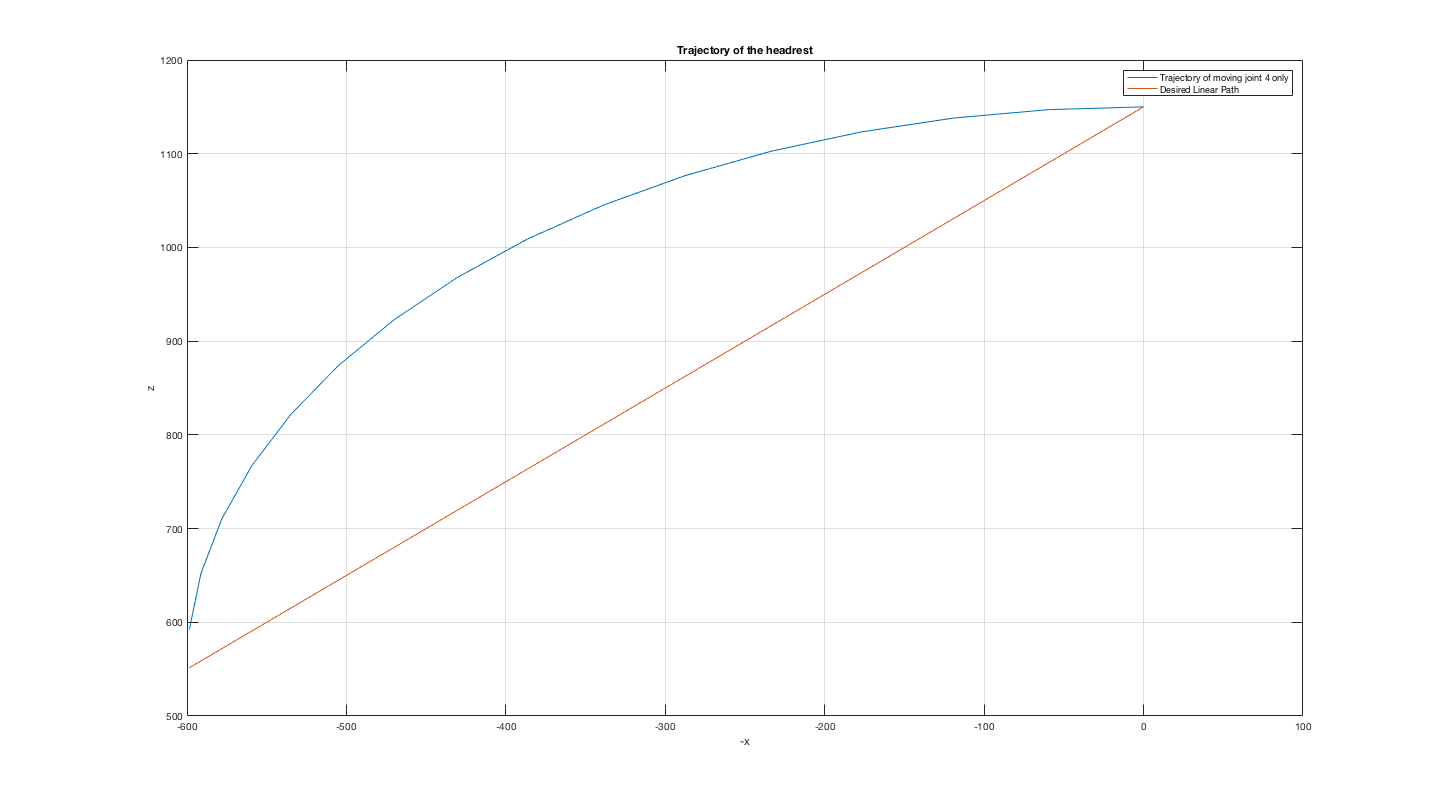
\includegraphics[scale=0.35]{traj1}
  \caption{Trajectory Analysis}
  \label{fig:2}
\end{figure}
As can be seem from the figure, the blue path travels longer distance than the red path (linear). In a lots of applications, the linear path is more desirable. To achieve this, we make use of inverse kinematics. First, we compute the equation for the linear path, two points (0, 1150), (600, 550)
\begin{align*}
  z - 1150 &= -1 (x) \\
  z &= -x + 1150 
\end{align*}
Once we get this equation, we can increment x, find z from the equation, such that we have different points along the linear path we want to be. Next, we pass each point to the IK function, get each joint parameters q in each state, update q, then pass the next x and current state q in the inverse function. By the end of this process, we can get a list of q in each state. Passing this list of q into our FK function should give us the desired linear trajectory we want. Increasing the number of increments will make the trajectory more and more linear. The attempted code is shown in Result.m Section 3: Trajectory using IV, though not too successful.

\section{Collaboration}
I worked with Amir Omidfar and Angel Jimenez for the most part of the project, including coming up with the model, drawing schematics, figuring out the DH parameters, and implement FK and IK in Matlab. The work done are distributed equally between three of us, each having 1/3. \par
This lab is easily the most difficult lab I have ever worked on in UCLA. Spent 2 nights (including one all-nighters) for a total time more than 15 hours. I found the first section relatively easier but it just goes south from there. A lots of the time are spent to fully understand the material covered in this class. The most fun part of this lab is I got to work with a team: exchanging ideas and learn together. Lastly, I would like to say this lab is challenging and at the same time truly rewarding.

\end{document}
%==================================================%
% Bibliography starts here
%==================================================%
% \bibliographystyle{unsrt}
% \bibliography{my_latex_math_template}

%%% Local Variables:
%%% mode: latex
%%% TeX-master: t
%%% End:
